\documentclass[10pt,twocolumn,letterpaper]{article}

\usepackage{cvpr}
\usepackage{times}
\usepackage{graphicx}
\usepackage{amsmath}
\usepackage{amssymb}
\usepackage{url}
\graphicspath{ {./images/} }

\usepackage[breaklinks=true,bookmarks=false]{hyperref}

\cvprfinalcopy

\begin{document}

%%%%%%%%% TITLE
\title{COMPUTER VISION BASED ATTENDANCE SYSTEM}

\author{ANANDHINI RAJENDRAN\\
IIIT HYDERABAD\\
Professor CR Rao Rd, Gachibowli, Hyderabad, Telangana 500032\\
}

\maketitle

%%%%%%%%% ABSTRACT
\begin{abstract}
    This paper is about the automatic attendance management using facial recognition. The automatic attendance management will replace the manual and bio metric method, which takes a lot of time in class and has many loopholes like students leaving class after attendance. There are many bio metric processes ~\cite{biometric}, in that face recognition is the best method. In this paper we are going to describe the attendance without human interference. In this method first we create a database for students and professors which can be linked to their moodle/organisation website provided to them. In the next step we use face recognition software like YOLO ~\cite{yolo}, FaceNet ~\cite{facenet1} to detect and extract them. Then we run face matching algorithms like Siamese networks~\cite{face-detect}. Finally we mark attendance and set up reasons column for students to fill up their reason for absence and professor can either approve or disapprove leavs.
\end{abstract}

%%%%%%%%% BODY TEXT
\section{Introduction}

Maintenance of student attendance is the most difficult task in various institutions. Every institution has its own method of taking attendance such as using attendance sheet or by using some biometric methods. But these methods consumes a lot of time. There are many biometric methods available in which the basic concept is same. One of them is the finger print identification. In this method first the finger prints of the individuals are collected and stored in the database of finger print sensor. But this method has a flaw that students leave after giving attendance and some come to class only after attendance arrives. Hence, these attendance system, are not guaranteed and reliable.

Hence we address this issue by bringing up an automated attendance software based on face recognition. This is based on existing face recognition and detection algorithms. The recorded data is stored in database and hence easy to access and update. All the information of attendance by course and per student can be easily retrieved. This helps in accurate information and automation reduces manual time for attendance. This also helps students to plan their leaves according to the attendance shown in database and professors can also approve leaves which makes even leave application more effective. Earlier leave applications required that the professors must be informed separately but this reduces the work.



%------------------------------------------------------------------------
\section{Literature Review}

There are numerous applications and people working on this idea.



There are many apps that have been using facial recognition system for online classes such as Axonator- touch free employee attendance app based on facial recognition technology. The Axonator employee attendance app is also equipped with voice detection feature that makes the entire system of marking attendance touch-free.It also generates report automatically.

Attendance Monitoring System using Face Recognition paper 
method for Student’s Attendance System which will integrate
with the face recognition technology using Personal
Component Analysis (PCA) algorithm. The attendance will be
marked based on facial recognition of the person. A group
image of the class will be captured and detected faces are
segmented from the captured image. The segmented faces are
then compared with a predefined database of all the students
of the class. The matlab code has already been built.But research is still going on to improve performance and general images.~\cite{software}

Face++ has software to detect face,compare faces and face searching.It also allows metadata obtained to be stored and returns collection for similar faces.It can be used in both mobile and web API.~\cite{face++}

Most of the apps are limited to online sources and not for offline classrooms. Research is still going on for large distance detection's.

%------------------------------------------------------------------------
\section{System Architecture}


The key components of this project:
\begin{center}
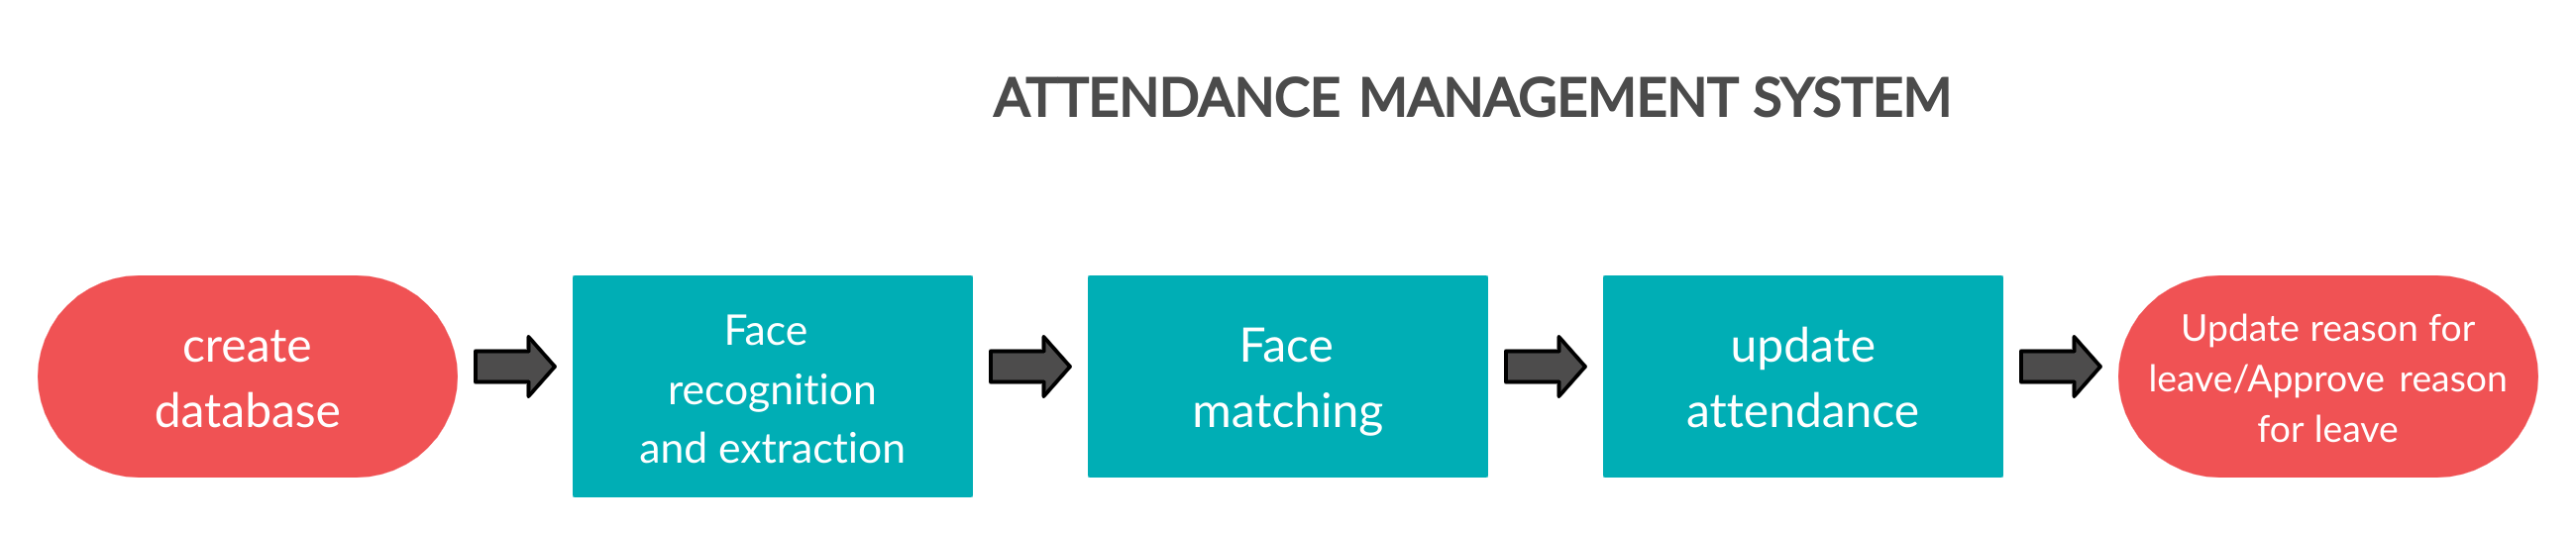
\includegraphics[width=1\linewidth]{images/1.png}
\caption{Figure 3 KEY COMPONENTS OF THE SOFTWARE SYSTEM}
\end{center}

1. Creating a database - Creating a my SQL database which keeps record of attendance.There are 2 tables for student and professor with features for student table as student-id, course-id(multiple valued key), face-id(id generated corresponding to one's face, attendance, and reason fields and professor table with professor-id, teaching-course-id(multiple valued key), attendance of course, and approve reason field.After each class the attendance of students will be updated in both tables and student can fill up the reason for absence.Then the professor decides if reason is approved or not and can update if approved.When the professor approves reason the attendance of student changes.The database can be linked to the organisation's website or the individual website which already exists.The use case diagram for this is given in the below figure 3.1.
\begin{center}
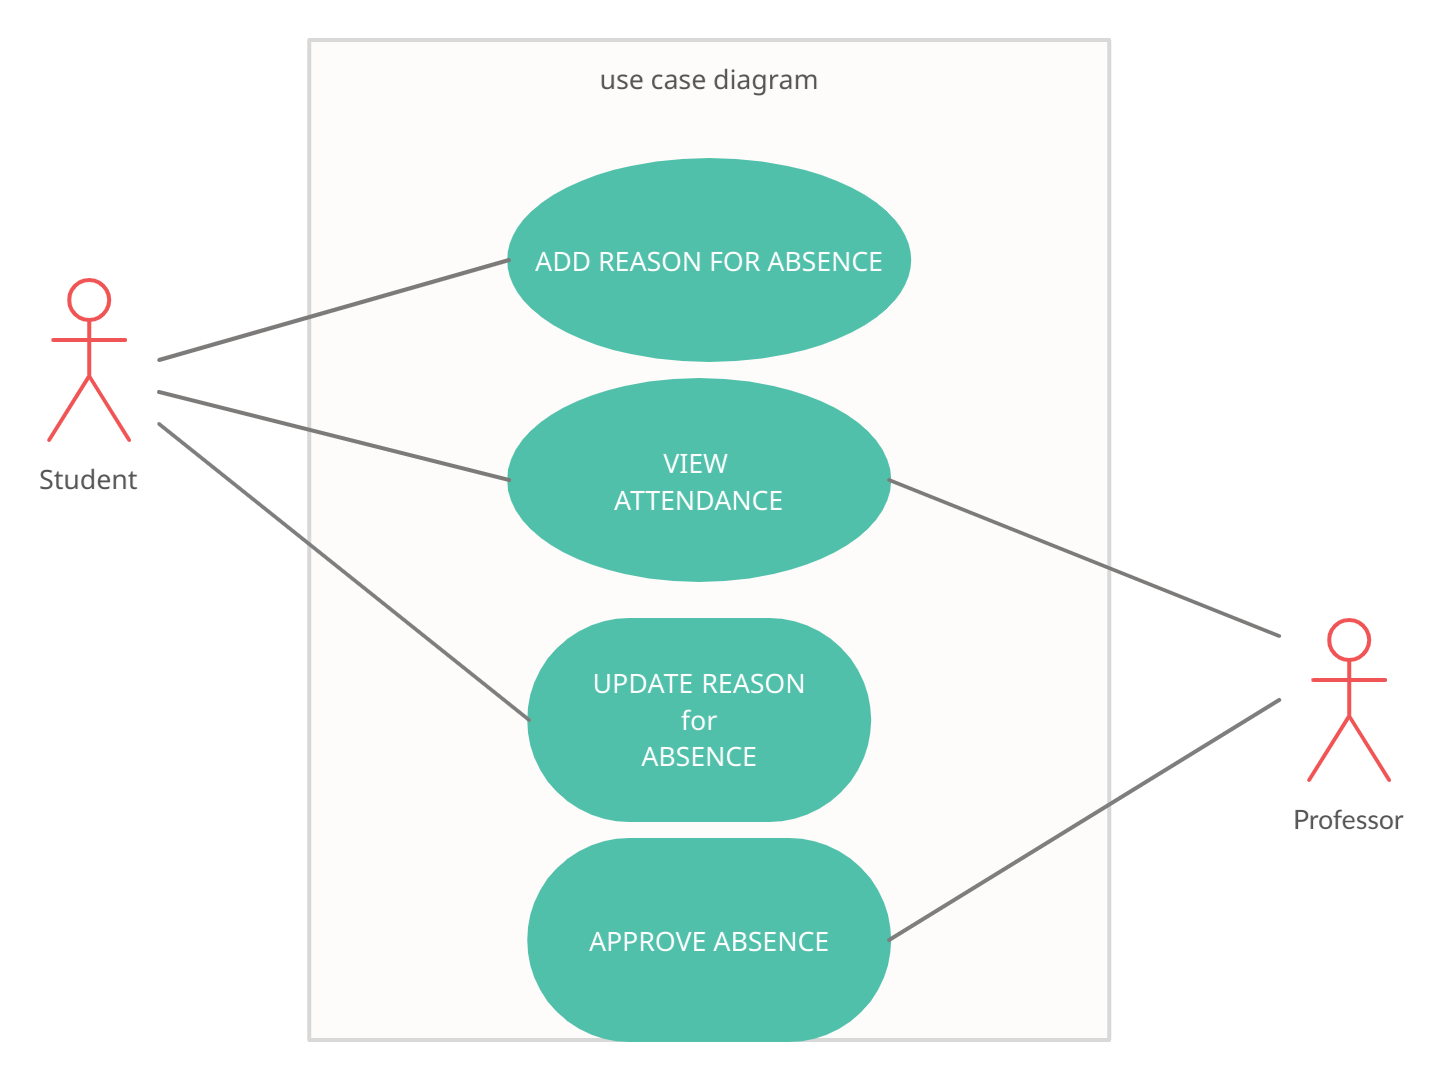
\includegraphics[width=1\linewidth]{images/use_case_diagram.png}
\caption{Figure 3.1. Use Case Diagram}
\end{center}

2. Face detection and extraction -  Face detection can be done using various face recognition software's like Yolo ~\cite{yolo}, Facenet ~\cite{facenet1}, etc.Once the faces of students are detected~\cite{facedetect} and extracted using any method for example, using convolution neural networks and K-nearest neighbour algorithm~\cite{face-detect}.

FaceNet is a face recognition system developed in 2015 by researchers at Google that achieved then state-of-the-art results on a range of face recognition benchmark data-sets.The FaceNet system can be used to extract high-quality features from faces, called face embedding, that can then be used to train a face identification system.~\cite{facenet}

To reduce the time for detecting face we can use half face detection template i.e since most human faces are symmetrical we only check for detecting half face.~\cite{facedetect}

We can use face recognition similar to bio metrics, there are algorithms that are able to handle a wide range of variations in static colour images, based on lighting compensation techniques, various skin tones and with very complicated background and uses signature of the different skin regions identified to uniquely identify the face candidates.~\cite{facedetect2}

\begin{center}
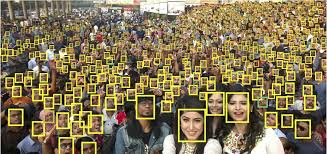
\includegraphics[width=1\linewidth]{img1.jpeg}
\caption{Figure 3.2 Face detection using Yolo}
\end{center}

3. Face matching - Face matching is done to check if the student in the course is present in the room or not. Student's image is taken when he is enrolled in a course and continuous face matching will also tell the duration of a student in the class.

We can use face detection algorithms like Siamese networks which are based on convolutional neural networks and calculate the degree of similarity between images.~\cite{face-matching}


This can also be used to monitor if student is paying attention or not e.g. closed eyes or lying on desk. With the increase in accuracy of algorithms this also can be implemented for strict monitoring for exams.

\begin{center}
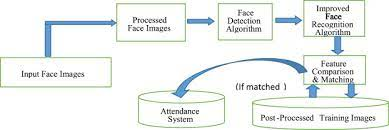
\includegraphics[width=1\linewidth]{images/face_mathcing.jpeg}
\caption{Figure 3.3 Face detection and matching for attendance system }
\end{center}


4. Marking attendance -  Once the faces are matched then the software returns the ids of students present in the class and hence updating the database using the id(primary key). Then students can write reasons for absence in the reasons column and the cumulative absent student names and reasons will be sent to the professor of the course.(course id is made foreign key here so it updates automatically).The professor can approve i.e. tick the reasons which are considered valid and the marked reasons corresponding student id's attendance will me marked present.

We can also make an automatic reason eliminator i.e eliminate the reasons apart from medical and travel issues.So that the professor
need not see all reasons and might be a time consuming schedule. For leaves approved by the institute the link to the approved document can be attached and an automatic checker can be designed e.g. a simple python code to check for strings like the institute name, approved sign, leave approved lines, etc.


 %------------------------------------------------------------------------
\section{Conclusion and Future Work}

This paper introduces the efficient method of automated attendance management system in the classroom
environment that can replace the old manual methods. No need for specialized hardware for
installing the system in the classroom. It can be
constructed using a camera.This system automatically updates and manages attendance in a procure manner. Maintaining attendance automatically with the help of face recognition will be very helpful and less prone to errors as compared to manual process. This will also reduce manipulation of attendance record done by students.
as well. 
Future scope - A mail which contains the information about absent as well as attendance percentage is mailed to the respective students using automated face recognition based attendance management system. This system can also be extended to monitoring examinations using more accurate facial expression detection algorithms.


{\small
\bibliographystyle{ieee}
\bibliography{references}
}

\end{document}